

\documentclass[10pt,twoside,slovak,a4paper]{article}

\usepackage[slovak]{babel}
\usepackage[IL2]{fontenc} 
\usepackage[utf8]{inputenc}
\usepackage{graphicx}
\usepackage{url} 
\usepackage{hyperref} 

\usepackage{cite}

\pagestyle{headings}

\title{Vývoj, využitie a zdokonaľovanie Non-Player Characterov v hrách\thanks{Semestrálny projekt v predmete Metódy inžinierskej práce, ak. rok 2022/2023, vedenie: Ing. Igor Stupavský}}

%\title{Vývoj, využitie a zdokonaľovanie Non-Player Characterov v hrách}


\author{Peter Pipasík\\[2pt]
	{\small Slovenská technická univerzita v Bratislave}\\
	{\small Fakulta informatiky a informačných technológií}\\
	{\small \texttt{xpipasik@stuba.sk}}
	}

\date{\small 18. október 2022}

\begin{document}

\maketitle

% lepsie by bolo dat to opacne abstrakt a uvod... lebo uvod sa viac podoba abstraktu
% pretoze ten abstrakt pripomina skor uvod... nie je pisany tak ako by mal abstrakt byt pisany .....

\begin{abstract}
Postavy neovládané hráčom (po anglicky non-player character, skrátene NPC) sa bezpochyby stali súčasťou hier a herného sveta v modernej dobe. Každý z nás vníma tieto postavy ako samozrejmosť no nikto z nás sa nezamyslí nad tým ako by hry vyzerali bez postáv neovládaných hráčom. V tomto článku sa pokúsim dokázať že herný svet by nemohol existovať
bez týchto postáv a aj keby existoval nebol by tak zaujímavý a napínavý. Poukážem na to že moderné počítačové, konzolové a mobilné hry by bez postáv typu NPC skoro zanikli.
   

\end{abstract}

\section{Úvod}
V tomto článku sa budem snažiť obecne objasniť pojem NPC (časť~\ref{Vyznam skratky}). Mojou prioritou bude vysvetlenie základov fungovania NPCs v hrách a ich využitie. Následne sa budem snažiť odvodiť dôležitosť týchto postáv v moderných hrách (časť~\ref{Dolezitost}). Budem sa teda snažiť dokázať že moderné hry už nie sú schopné fungovať bez týchto postáv. Teoreticky odvodiť nemožnosť vytvorenia hry bez postáv typu NPC.
Obecné objasnenie pojmu NPC bude obsahovať vznik (časť~\ref{Vznik}) a využitie NPCs ale taktiež aj priblíženie čo je to NPC na základnej úrovni, teda jednoduché a jasné vysvetlenie základných pojmov spojených so slovným spojeným non-player character (časť~\ref{Vyznam skratky}).
K záveru chcem čitateľovi priblížiť pokrok za posledné roky (časť~\ref{Rozvoj}). Presnejšie povedané históriu NPCs v hrách a pokrok vo vytváraní NPCs. Celkový pokrok obsahuje napríklad zlepšenie interakcie hráča s NPC postavou a rozvoj osobnostných čŕt pre NPCs. 


\section{Význam skratky NPC}  \label{Vyznam skratky}
Skratka NPC je odvodená z pojmov: Non-Player Character, Non-Player Class a taktiež Non-Playable Character. Jedná sa teda o nehráčsku alebo nehrateľnú postavu. Ako NPC sa považuje akákoľvek postava v hre ktorú neovláda hráč ale je ovládaná pomocou počítača teda ovláda ju samotná hra, herná mechanika a umelá inteligencia danej hry \cite{Hack2018}. V modernejších hrách má každá nehrateľná postava svoju vlastnú umelú inteligenciu. NPC má vopred určený súbor správania ktorý ovplyvňuje vyhodnocovanie daných situácií. NPC sa vyskytuje prevažne v hrách typu RPG (Role Playing Game) a MMORPG (Massively Multiplayer Online Role Playing Game) \cite{9291553}.


\section{Vznik NPC}    \label{Vznik}
\subsection{Prvý výskyt NPC} \label{NPC 1 time}
Odpovedať na otázku ktorá hra bola úplne prvou hrou obsahujúcou úplne prvé NPC je náročné. Niekto by mohol povedať že to bola hra Bertie the Brain z roku 1950 no však táto hra neobsahovala žiadne postavy. Určitá skupina ľudí považuje za prvú hru obsahujúcu NPC hru Space Invaders z roku 1978. Táto hra je považovaná za jednu z prvých hier ktorá bola schopná splniť minimálne požiadavky na to aby mohla byť klasifikovaná ako hra obsahujúca NPC. Pointa hry bola jasná a jednoduchá a to zostreliť všetky mimozemské lode ktoré postupne klesali nižšie. Tieto mimozemské lode sú určitou skupinou ľudí vnímané ako úplne prvé NPC v hrách, nakoľko hráč nemal možnosť ich ovládať a svojim spôsobom sa jednalo o postavy a nie len o umelú inteligenciu ako v prípade Bertie the Brain. 


\subsection{Prvé NPCs, Pac-Man}
Prvými skutočnými a väčšinou prijatými NPCs boli štyria duchovia z hry Pac-Man (Namco, 1980). A to Blinky, Pinky, Inky a Clyde. Každý z týchto štyroch duchov má svoje vlastné individuálne vzory pohybu. Vzormi pohybu sú myslené spôsoby ako sa daný duch pohybuje po mape hry. Každý z duchov má svoje vlastné primitívne a veľmi jednoduché algoritmy. \cite{Hack2018}
 



\section{Typy NPCs}     \label{Typy}
V hrách sa často stretávame s mnohými NPCs ktoré sa prevažne delia na 3 typy a to priateľské NPCs (časť~\ref{Ally & non}), neutrálne NPCs (časť~\ref{Ally & non}) a nepriateľské NPCs (časť~\ref{enemy}). Každá z týchto skupín má predom určenú úlohu a vopred určený význam v hre. Samozrejme záleží aj na príbehu danej hry. Tieto 3 typy sa dajú pokladať ako jedno z úplne základných rozdelení pre NPCs, pretože každý typ sa v závislosti na danej hre ešte ďalej rozvetvuje. Keďže každá hra je iná a v každej hre sa nachádzajú parametrálne odlišné NPCs som sa rozhodol opísať význam, správanie, dôležitosť a hlavnú funkciu najčastejšie sa vyskytujúcich podskupín. (Názvy podskupín boli inšpirované článkom \cite{phdthesis})

\subsection{Priateľské a neutrálne NPCs}  \label{Ally & non}  

\subsubsection{Civilisti} 
Civilisti v hrách majú jednu jedinú špecifickú úlohu a to vyplniť priestor aby mal hráč pocit že je vo svete ktorý skutočne žije. Ak je hráč v dostatočnej blízkosti NPC typu civilista zväčša má možnosť opýtať sa ho náhodnú otázku, pozdraviť ho alebo ho okradnúť v niektorých hrách ho dokonca aj zabiť. V prípade otázky a pozdravu od hráča mu NPC odpovie jednu z vopred naprogramovaných odpovedí. NPCs typu civilista sa prevažne vyskytujú v civilných oblastiach ktoré sa majú podobať mestám a dedinám v skutočnom živote.  


\subsubsection{Obchodníci}
NPCs typu obchodník slúžia hráčovi k nákupu zbraní, munície, máp a rôznych dekoračných premetov. Dalo by sa o nich povedať že plnia rolu predavača z reálneho sveta. Občas sú aj poskytovatelia služieb na vylepšenie hráčovej postavy. Tieto NPCs sú nesmierne dôležité pre každú hru. Niektoré hry obsahujú typ NPC ktorý plní rolu barmana, predajcu áut, predajcu pozemkov. Vo väčšine hier taktiež existuje typ obchodníka, ktorý poskytuje výmenu jeho inventáru za hernú menu. Vďaka hernej mene je hráč schopný nakúpiť si vyššie spomenuté predmety.  


\subsubsection{Poskytovatelia úloh, výziev a misií}
NPC typu poskytovatelia úloh, výziev a misii slúžia na rozrastenie hlavného a aj vedľajšieho príbehu hry. Sú to postavy ktoré slúžia aj ako poskytovatelia základných informácií ohľadom histórie, tradícií a lokalít. Niektoré misie a výzvy nemusia súvisieť s príbehom hry, majú za úlohu hráča pobaviť a poskytnúť mu predmety k vylepšeniu postavy, aby mal hráč možnosť ľahšieho postupu hrou. 


\subsubsection{Strážcovia a bojovníci} \label{services}
NPC typu strážcovia a bojovníci sú spoločne s pešiakmi (časť ~\ref{Pesiaci}) jedným s najpočetnejšie zastúpenými NPCs v hrách. Sú na strane hlavného hrdinu (hráča) ale môžu byť aj proti hráčovi ak hráč robí zlé veci ako napríklad zabíjanie nevinných civilistov, kradnutie a podobné. Pomáhajú hráčovi dobývať územie a postupovať ďalej v hre. Po dobytí územia ho väčšinou začnú ochraňovať a žiť na danom území. Hráč má možnosť s nimi vytvárať vzťahy a tým pádom sa viac vcítiť do hry.  Ak hráč pomôže týmto NPC postavám je väčšinou odmenený napríklad: muníciou, novými zbraňami, zberateľskými predmetmi, hráčskou menou (peniazmi) poprípade zľavou na predmety v hernom obchode. V niektorých hrách má hráč možnosť najať si vlastného žoldniera ktorý mu bude pomáhať postupovať v hre.    

\subsubsection{Zvieratá}
NPC typu zvieratá majú podobný účel ako NPC typu civilista teda jednou z ich hlavnou úlohou je zaplniť herný svet. Rozdeľujú sa na viaceré typy ako napríklad ochranné zvieratá (pes, mačka), bojové zvieratá (lev, medveď), prepravné zvieratá (kôň) a zvieratá určené ako potrava pre hráča (ryby a dobytok). Je možné s nimi interagovať napríklad pohladkať ich alebo ich nakŕmiť. 

\subsection{Nepriateľské NPCs} \label{enemy}

\subsubsection{Hlavný protivník (Villain)} \label{BOSS}
Hlavný záporák (po anglicky Villain) je špecifický typ NPC. Jedná sa zväčša iba o jednu jedinú postavu v hre ktorá tvorí veľkú časť hlavného príbehu celej hry. Charakteristické črty tohto NPC sú: túžba po moci, snaha ukrivdiť hlavnému hrdinovi, hlavným cieľom je zväčša ovládnutie herného sveta a teda dobytie a nadvláda, hnaný pomstou. Zabitie tohto NPC vo väčšine hier znamená koniec hry (príbehovej časti hry).

\subsubsection{Boss} \label{BOSS}
Boss je typ NPC ktorý je podobný ako NPC typu Villain. Má rovnaké charakteristické črty ako Villain s tým rozdielom že NPC typu Boss je poddaný hlavnému záporákovi teda tento typ NPC chce získať slávu a rešpekt u svojho pána (hlavného záporáka) čo v hrách často vyústi k tomu že Boss je ochotný obetovať svoj život v súboji s hlavným hrdinom (hráčom). Po ich zabití sa hlavná dejová línia hry nekončí väčšinou sa po ich zabití posúvame do ďalšej fázy hry (niekedy aj do inej mapy) kde na nás čaká iný Boss. Po zabití posledného Bossa býva väčšinou súboj s hlavným záporákom. Po zabití Bossa hráč obdrží špecifické predmety ktoré mu majú pomôcť v ďalšom postupe hrou. 

\subsubsection{Pešiaci} \label{Pesiaci}
Pešiaci tvoria jedno z najmohutnejších zastúpení postáv typu NPC v hrách. Jedná sa prevažne o žoldnierov, nepriateľskú armádu, nepriateľských lukostrelcov; tažkoodencov;  mágov alebo lovcov. Slúžia ako nástroj pre hlavného záporáka poprípade Bossa. Zväčša nejednajú z vlastnej vôle iba plnia rozkazy. Delia sa na rôzne skupiny ako napríklad gangy. V hre plnia úlohu zábavy pre hráča. Ich herné opodstatnenie je zaplnenie herného sveta, poukázanie na to že v tomto hernom svete je potrebné zastaviť hlavného záporáka a jeho nasledovateľov.  

\subsubsection{Ostatný nepriatelia} \label{Ostatny_nepriatelia}
NPC typu ostatný nepriatelia sa v každej hre líšia. Napríklad v hre The Witcher 3: Wild Hunt (CD Projekt RED, 2015) sú to monštrá ktoré sa ďalej delia na rôzne skupiny monštier ako napríklad: griffin, siréna, drak, upír, vlkolak, škriatok a iné.  Vyššie spomenutý ostatný nepriatelia sa však nemusia nachádzať v iných hrách alebo sa v nich nachádzajú ale v inom prevedený. K tomuto typu môžu patriť aj zvieratá ktoré nie sú neutrálne/ priateľské.


\section{Dôležitosť charakterov NPC pre hry a herný priemysel}   \label{Dolezitost}

Postavy typu NPC sú pre herný priemysel a samotné hry nesmierne podstatné a to z dôvodu marketingu a dopytu ale zároveň pre ich schopnosť vytvárania deju hry. Samozrejme NPCs sú v modernej dobe neodmysliteľnou súčasťou hier a herného priemyslu. Avšak existujú aj hry ktoré neobsahujú postavy typu NPC a aj napriek tomu sú úspešné. Tým pádom by sme mohli konštatovať že pre hry a herný priemysel postavy typu NPC nie sú dôležité a podstatné ale tieto hry tvoria percentuálnu menšinu.%dorobit a zmenit nazov  

\subsection{Všeobecný význam a prínos charekterov typu NPC}

\subsubsection{Dej hry}
Bez existencie postáv typu NPC by nemohli existovať tituly ako MMO,MMORPG a mnohé ďalšie 
ktorých hlavnú črtu hry tvorí príbeh. Príbeh v hrách nie je možné vytvoriť bez pomoci postáv typu NPC. 
Teda ak by postavy typu NPC neexistovali žánre závislé na deji by tým pádom zanikli. 
Bez deju by hra stratila svoje čaro a hráč by sa len bezducho potuloval svetom. Aj napriek tomu 
existujú hry ktorých dej je druhoradý dalo by sa povedať až skoro nulový ako 
napríklad hra s názvom Minecraft (Mojang, 2009). No aj napriek nedostatku príbehu 
táto hra ponúka nespočetné množstvo NPCs typu zvieratá, obchodníci, bossovia a iný typ nepriateľov.

\subsubsection{Výplň sveta a pohľad na skutočný svet}
NPCs pomáhajú zaplniť herný svet a dať hráčovi pocit že je vo svete ktorý,
skutočne žije. Dôkazom tohto tvrdenia je aj tabuľka počtu postáv typu NPC v hre The Witcher 3: Wild Hunt (CD Projekt RED, 2015). Táto hra vyhrala The Game Awards 2015 a teda sa stala najúspešnejšou hrou roku 2015. 


\begin{center}

\hfill \break
    
\begin{tabular}{|c|c|}
    
     \hline
     Typ postavy NPC & Počet\\
     \hline
     vedlajšia postava & 65\\
    \hline
    monštrum & 80\\
    \hline
    zviera & 31\\
    \hline
    priateľ a nepriateľ &389\\
    \hline

\end{tabular}

\hfill \break

\end{center}




Čím reálnejšie pôsobí postava typu NPC tým viac sa dokáže hráč do tejto postavy vcítiť a prežívať emócie s touto fiktívnou postavou. Emócie sú nesmierne dôležité pretože dokážu ponoriť hráča do hry a umožnia mu prežívať tento fiktívny svet ako reálny. Dobre napísané postavy typu NPC dokážu mať veľmi veľký morálny význam a dokážu ovplyvniť hráčov a teda aj skutočný svet. Niektoré hry a postavy majú hlbší zmysel než len pobaviť hráča a teda vďaka nim sa daný hráč začne pozerať na skutočný svet inak. Mnohé problémy ktoré riešia NPCs v hrách sú podobné ako tie v skutočnosti. Tým pádom dokážu pomôcť hráčom s ich problémami v skutočnom svete. 

\subsection{Marketing a dopyt}
Realistickejšie postavy typu NPC majú za následok vžitie sa hráča do herného sveta. Teda hráč strávi viac času v hre a tým pádom má hra viac priestoru na následné mikrotransakcie. Mikrotransakcie sú nesmierne dôležité pre marketing či už sa jedná o nákup skinov pre hlavnú postavu, nákup skinov na zbrane, zakúpenie si novej zbrane do hry alebo nákup hernej meny. Miktortansakcie sú neodmysliteľnou súčasťou herného priemyslu. 
Ak by si hráč nič v danej hre aj napriek tomuto nezakúpil tým že hrá hru častejšie jej zvyšuje percentuálnu hrateľnosť a teda daná firma ktorá, stojí za touto hrou má lepší rating.



\section{Pokrok a rozvoj}  \label{Rozvoj}

Za posledných niekoľko desaťročí došlo v hernom priemysle k obrovskému vzrastu. Hlavný vzrast a pokrok je viditeľný hlavne vo vylepšení grafiky, hrateľnosti a aj zvuku. No bohužiaľ vývoj umelej inteligencie a postáv typu NPC nepostupoval rovnakým tempom. Aj keď bezpochyby došlo k určitým zlepšeniam vo vývoji NPCs stále tento pokrok zaostáva za grafikou a inými aspektami spojenými s herným priemyslom a hrami samotnými. \cite{phdthesis})

Spôsob vývoja a zmýšľania NPCs sa za posledné roky veľmi nezmenil. Merateľný pokrok je viditeľný len z dekády na dekádu. NPCs od doby hier ako bol napríklad Pac-Man určite prešli značne viditeľným a zásadným pokrokom no ale v modernej dobe je zmena a teda následný pokrok NPCs v hrách a hernom priemysle z roku 2015 a 2022 pre bežného hráča neexistujúci. Postavy typu NPC v poslednej dekáde neprešli veľkou a zásadnou zmenou a stále sa riadia jednouchými predom zadanými súbormi príkazov. \cite{9730383}  

\subsection{Strom rozhodovania}
Pri NPCs je veľmi dôležité pred ich samotným naprogramovaním vedieť ako by mali reagovať na určité situácie ktoré môžu v hre nastať. Strom rozhodovania nám na diagrame ukazuje ako by sa malo správať určité NPC v danej situácii. \cite{9291553} Existuje aj dialógový strom ktorý slúži na reprezentáciu možných dialógov hráča s NPC. Tieto mechanizmy sa využívajú v mnohých hrách a sú dôležité pre správnu interakciu hráča s NPC.

V svojej podstate ide len o jednoduchý If/Else algoritmus pre ktorý je potrebné predom vedieť čo má byť podmienka a čo sa má vykonať ak je podmienka pravdivá alebo nepravdivá. 

\graphicspath{MIP_NPC_latex}

\begin{center}

\hfill \break

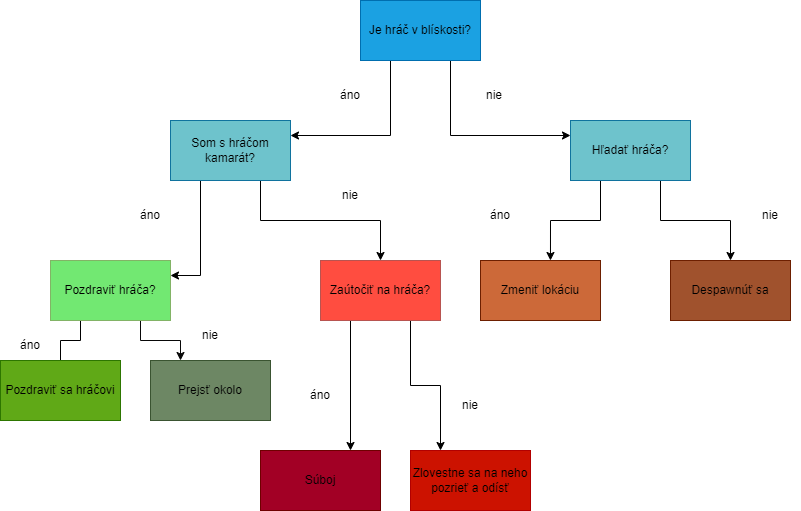
\includegraphics[scale = 0.40]{MIP_NPC_latex.png}

\hfill \break

\end{center}

\section{Záver...}

% z tadeto sa cerpa

\bibliography{NPC_literatura}
\bibliographystyle{alpha}

% sem bude treba dat moj nazor na temy z prednasok...

\end{document}
